%!TEX root = /Users/audrey/Dropbox/PhD/MOMAB/ArXiv/Latex/paper.tex

\section{Multi-Objective Bandits}
\label{sec:momab}

A multi-objective bandits problem is described by a (finite) set of actions $\cA$, also referred to as the \emph{design space}, each of which is associated with a $d$-dimensional expected outcome $\bsmu_a = (\mu_{a, 1}, \dots, \mu_{a, d}) \in \cX \in \Real^d$. For simplicity, we assume that the \emph{objective space} $\cX = [0, 1]^d$. In this episodic game, an agent interacts with an environment characterized by a \emph{preference function}~$f$. The agent iteratively chooses to perform an action $a(t)$ and obtains a noisy observation of $\bsz(t)$.\footnote{Scalars are written unbolded; vectors are boldfaced. The operators $+$, $-$, $\times$, and~$\div$ applied on a vector $\bsv = (v_1, \dots, v_d)$ and a scalar $s$ correspond to the operation between each item of $\bsv$ and $s$, e.g., $\bsv + s = (v_1 + s, \dots, v_d + s)$. These operators applied on two vectors $\bsv = (v_1, \dots, v_d)$ and $\bsu = (u_1, \dots, u_d)$ correspond to itemwise operations between $\bsv$ and $\bsu$, e.g., $\bsv + \bsu = (v_1 + u_1, \dots, v_d + u_d)$.}

An algorithm for a multi-objective bandits problem is a (possibly randomized) method for choosing which action to play next, given a history of previous choices and obtained outcomes, $\cH_t = \{ a(s), \bsz(s) \}_{s = 1}^{t-1}$. Let $\cO = \argmax_{a \in \cA} f(\bsmu_a)$ and let $\star \in \cO$ denote the optimal action. The optimal gap $\Delta_a = f(\bsmu_\star)- f(\bsmu_a)$ measures the expected loss of playing action $a$ instead of the optimal action. The agent's goal is to design an algorithm with low expected (cumulative) regret\footnote{Also known as the scalarized regret~\cite{Drugan2013}.}:
\begin{align}
\label{eqn:regret}
    \kR(T)
    = \sum_{t=1}^T \big( f(\bsmu_\star) - f(\bsmu_{a(t)}) \big)
    = \sum_{t = 1}^T \sum_{a \in \cA} \Pr[a(t) = a] \Delta_a.
\end{align}
This quantity measures the expected performance of the algorithm compared to the expected performance of an optimal algorithm given knowledge of the outcome distributions, i.e., always sampling from the distribution with the expectation maximizing $f$. Typically, we assume that the algorithm maintains one estimate $\bstheta_a(t)$ per action $a$ on time $t$. Let $\cO(t) = \argmax_{a \in \cA} f(\bstheta_a(t))$ denote the set of actions with an estimate maximizing $f$. The algorithm faces a trade-off between playing an action $a(t) \in \cO(t)$ and choosing to gather an additionnal sample from a relatively unexplored action in order to improve its estimate. Alg.~\ref{alg:mobandits} describes this multi-objective bandits problem.

\begin{algorithm}[t]
    On each episode $t \geq 1$:
    \begin{enumerate}[nolistsep]
        \item The agent selects action $a(t)$ to play given $\cO(t)$.
        \item The agent observes $\bsz(t) = \bsmu_{a(t)} + \bsxi(t)$, where $\bsxi(t)$ are i.i.d. random vectors.
        \item The agent updates its estimates.
    \end{enumerate}
    \caption{Multi-objective bandits setting}
\label{alg:mobandits}
\end{algorithm}

In many situations, the environment providing the preference function is a person, let us call her the \emph{expert user}. Unfortunately, people are generally unable to scalarize their choices and preferences. Therefore they cannot explicitely provide their preference function. However, given several options, users can tell which one(s) they prefer (that is $\cO(t)$) and thus can be used as a black box to provide feedback in the learning loop.
% Alg.~\ref{alg:mobandits_user} describes the user-guided multi-objective bandits problem.
%
% \begin{algorithm}[t]
%     On each episode $t \geq 1$:
%     \begin{enumerate}[nolistsep]
%         \item The agent selects action $a(t) \in \cO(t)$ to play.
%         \item The agent observes $\bsz(t) = \bsmu_{a(t)} + \bsxi(t)$, where $\bsxi(t)$ are i.i.d. random variables.
%         \item The agent updates its estimates.
%         \item The agent shows options $\{ \bstheta_a(t) \}_{a \in \cA}$ to the expert user.
%         \item The expert user indicates its preference $\cO(t) = \argmax_{a \in \cA} f(\bstheta_a(t))$.
%     \end{enumerate}
%     \caption{User-guided multi-objective bandits setting}
% \label{alg:mobandits_user}
% \end{algorithm}


\paragraph{Pareto-optimality}

Given two $d$-dimensional options $\bsx = (x_1, \dots, x_d)$ and $\bsy = (y_1, \dots, y_d)$, $\bsx$ is said to dominate, or Pareto-dominate, $\bsy$ (denoted $\bsx \succeq \bsy$) if and only if $x_i > y_i$ for at least one $i$ and $x_i \geq y_i$ otherwise. The dominance is strict (denoted $\bsx \succ \bsy$) if and only if $x_i > y_i$ for all $i = 1, \dots, d$. Finally, the two vectors are incomparable (denoted $\bsx \parallel \bsy$) if $\bsx \nsucc \bsy$ and $\bsy \nsucc \bsx$. Pareto-optimal options represent the best compromises amongst the objectives and are the only options that need to be considered in an application. We say that these options constitute the Pareto front $\cP = \{ a : \nexists \bsmu_b \succeq \bsmu_a \}_{a, b \in \cA}$. Fig.~\ref{fig:pareto_front} shows an example of dominated and non-dominated expected outcomes in a $d = 2$ objectives space. A user facing a multi-criteria decision making problem must select her preferred non-dominated option. Dominated options are obviously discarded by default.

\begin{figure}[t]
    \centering
    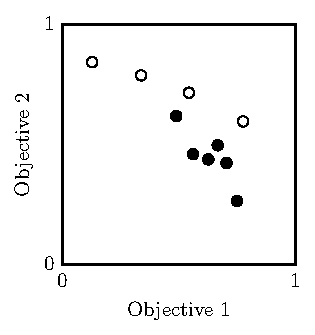
\includegraphics[scale=0.75]{pareto_front}
    \caption{Example of dominated (black) and non-dominated (white) options.}
\label{fig:pareto_front}
\end{figure}


\paragraph{Related Works}

The multi-objective bandits problem has already been addressed in the a posteriori setting, where the goal is to discover the whole Pareto front for a posteriori decision making~\cite{Drugan2013,Yahyaa2015}. This is different from the a priori optimization problem tackled here. The aim of algorithms in the a posteriori setting is to simultaneously minimize the Pareto-regret and the unfairness metrics. Also known as the $\epsilon$-distance~\cite{Laumanns2002}, the Pareto-regret associated with playing action $a$ is the minimum value $\epsilon_a$ such that $\bsmu_a + \epsilon_a$ is not dominated by any other actions. In other words, any action standing on the front is considered equally good by the expert user. This is like considering that $\cO = \cP$, which corresponds to the preference function $f(\bsmu_\star) = 1$, $f(\bsmu_a) = 1 - \epsilon_a$, such that $\Delta_a = \epsilon_a$. Note that any algorithm optimizing a single objective could minimize the Pareto-regret regardless of the other objectives. This is addressed by the unfairness metric, measuring the disparity in the amount of plays of non-dominated actions -- the idea being to force algorithms to explore the whole Pareto front evenly.

In MOO settings~\cite{Zuluaga2013}, the goal is to identify the Pareto-optimal set $\cP$ without evaluating all actions. The quality of a solution $\cS$ is typically given by the hypervolume error $V(\cP) - V(\cS)$, where the $V(\cP)$ is the volume enclosed between the origin and $\{ \bsmu_a \}_{a \in \cP}$ (and similarly for $\cS$). However, the hypervolume error does not give information about the quality of the estimation of actions. Identifying the Pareto front alone does not guarantee that the actions are well estimated and, therefore, that an expert user choice based on these estimations would lead to the right choice.
